\documentclass{szzclass}
\usepackage{hyperref}
\usepackage{longtable}
\usepackage{booktabs}

\subject{PSI}
\code{BI-SPOL-23}
\topic{ISO/OSI a TCP/IP model. Protokoly linkové vrstvy. Potvrzovací
metody. Přepínání a směrování. Principy fungování propojovacích síťových
prvků.}

\providecommand{\tightlist}{%
  \setlength{\itemsep}{0pt}\setlength{\parskip}{0pt}}

\begin{document}


% \hypertarget{spol-23-psi}{%
% \section{SPOL-23-PSI}\label{spol-23-psi}}

% \emph{ISO/OSI a TCP/IP model. Protokoly linkové vrstvy. Potvrzovací
% metody. Přepínání a směrování. Principy fungování propojovacích síťových
% prvků.}

\hypertarget{isoosi-model}{%
\section{ISO/OSI model}\label{isoosi-model}}

Tento model se osvědčil pro popis sítí a protokolů, ovšem univerzálním
standardem pro reálné sítě se nestal. Přišel ve špatnou dobu, nebyly
vhodné technologie a není žádná úspěšná implementace.

\begin{longtable}[]{@{}clll@{}}
\toprule
\# & Jméno vrstvy & Data & Funkce/protokol\tabularnewline
\midrule
\endhead
7 & Aplikační & Data & Komunikace s aplikací - SMTP, HTTP\tabularnewline
6 & Prezenční & Data & Reprezentace dat, komprese,
šifrování\tabularnewline
5 & Relační (session) & Data & Udržování relace\tabularnewline
4 & Transportní & Segments & End-to-end spojení - UDP,
TCP\tabularnewline
3 & Síťová & Packets & IP (logické adresování) - IP, IPX\tabularnewline
2 & Linková (data-link) & Frames & MAC (fyzické adresování) -
Ethernet\tabularnewline
1 & Fyzická & Bits & Bitový přenos - RS232, ADSL\tabularnewline
\bottomrule
\end{longtable}

\begin{figure}[h]
\centering
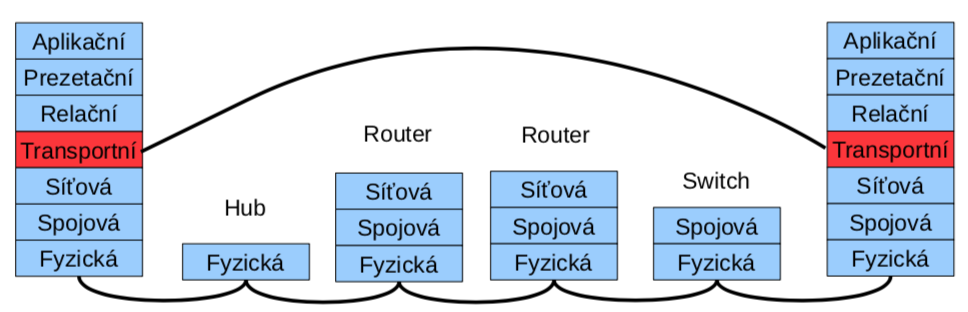
\includegraphics[width=\textwidth]{topics/bi-spol-23/images/ISO-OSI-Architektura.png}
\caption{Architektura ISO/OSI}
\end{figure}

\hypertarget{fyzickuxe1-vrstva}{%
\subsection{Fyzická vrstva}\label{fyzickuxe1-vrstva}}

\begin{itemize}
\tightlist
\item
  zajišťuje přenos bitů kanálem
\item
  definuje způsob přenosu 0 a 1 (napěťové vlastnosti, modulace)
\item
  definuje elektrické a mechanické vlastnosti média
\end{itemize}

\hypertarget{linkovuxe1-vrstva}{%
\subsection{Linková vrstva}\label{linkovuxe1-vrstva}}

\begin{itemize}
\tightlist
\item
  funkce spolehlivého spojení (detekce případně korekce chyb)
\item
  řízený přístup k lince (MAC - Medium Access Control)
\item
  řízení toku na lince
\item
  jednoznačná adresa v segmentu sítě (např. MAC v Ethernetu)
\item
  na této vrstvě pracují všechny bridge a switche
\end{itemize}

\hypertarget{suxedux165ovuxe1-vrstva}{%
\subsection{Síťová vrstva}\label{suxedux165ovuxe1-vrstva}}

\begin{itemize}
\tightlist
\item
  adresace a směřování dat přes mezilehlé prvky
\item
  síťová adresa - jednoznačná adresa v rámci celé sítě (např. IP adresa)
\item
  na této vrstvě pracují routery
\end{itemize}

\hypertarget{transportnuxed-vrstva}{%
\subsection{Transportní vrstva}\label{transportnuxed-vrstva}}

\begin{itemize}
\tightlist
\item
  rozklad dat na pakety
\item
  uspořádání paketů podle pořadí
\item
  multiplexuje a demultiplexuje data mezi jednotlivými spoji
\item
  transportní adresy (adresa, port)
\end{itemize}

\hypertarget{relaux10dnuxed-vrstva}{%
\subsection{Relační vrstva}\label{relaux10dnuxed-vrstva}}

\begin{itemize}
\tightlist
\item
  vytváření logického rozhraní pro aplikace
\item
  synchronizace spojení (transakce)
\item
  přihlášení, udržování relace
\item
  např. sdílení disků
\end{itemize}

\hypertarget{prezenux10dnuxed-vrstva}{%
\subsection{Prezenční vrstva}\label{prezenux10dnuxed-vrstva}}

\begin{itemize}
\tightlist
\item
  formátování a prezentace dat
\item
  transformace (komprese/dekomprese)
\item
  kódování (např. různé jazyky)
\item
  šifrování
\item
  např. ASCII/EBCDIC
\end{itemize}

\hypertarget{aplikaux10dnuxed-vrstva}{%
\subsection{Aplikační vrstva}\label{aplikaux10dnuxed-vrstva}}

\begin{itemize}
\tightlist
\item
  způsob komunikace aplikací - protokoly
\item
  podpůrné funkce aplikacím
\item
  představuje interface pro uživatele
\end{itemize}

\hypertarget{tcpip-model}{%
\section{TCP/IP model}\label{tcpip-model}}

Vznikl na akademické půdě, bez podílu komunikačních firem. Úspěšný
hlavně díky internetu. Model vnikl dodatečně, nejprve existovaly
protokoly.

Rozdíly oproti ISO/OSI: vynechány vrstvy prezenční a relační. A proběhlo
sloučení fyzické a linkové vrstvy.

Vrstvy:

\begin{longtable}[]{@{}cll@{}}
\toprule
\# & Jméno vrstvy & Jednotka na vrstvě\tabularnewline
\midrule
\endhead
4 & Aplikační & TCP segment\tabularnewline
3 & Transportní & IP datagram\tabularnewline
2 & Síťová & Ethernet frame\tabularnewline
1 & Síťové rozhraní & bity\tabularnewline
\bottomrule
\end{longtable}

\begin{figure}[h]
\centering
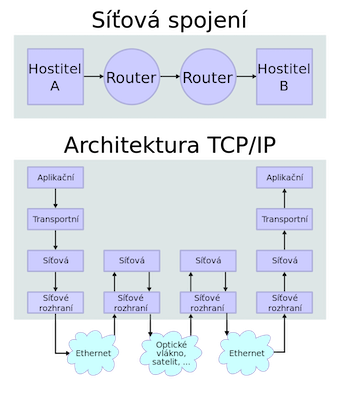
\includegraphics[width=\textwidth]{topics/bi-spol-23/images/TCP-IP-Architektura.png}
\caption{Architektura TCP/IP}
\end{figure}

\hypertarget{protokoly-linkovuxe9-vrstvy}{%
\section{Protokoly linkové
vrstvy}\label{protokoly-linkovuxe9-vrstvy}}

\begin{verbatim}
????????? TODO
\end{verbatim}

\hypertarget{potvrzovacuxed-metody}{%
\section{Potvrzovací metody}\label{potvrzovacuxed-metody}}

\hypertarget{pozitivnuxed-potvrzovuxe1nuxed}{%
\subsection{Pozitivní
potvrzování}\label{pozitivnuxed-potvrzovuxe1nuxed}}

\begin{itemize}
\tightlist
\item
  každý rámec musí být potvrzen (ACK)
\item
  pokud nedojde potvrzení do určitého času (timeout) je rámec odeslán
  znova
\end{itemize}

\#\#\#~Negativní potvrzování - přijímací strana potvrzuje - lze odeslat
i negativní potvrzení (NAK) - paket nedošel nebo je poškozen -
nepřijde-li ACK ani NAK uplatní se timeout

\hypertarget{ux10duxedslovuxe1nuxed-ruxe1mcux16f-frame-numbering}{%
\subsection{Číslování rámců (frame
numbering)}\label{ux10duxedslovuxe1nuxed-ruxe1mcux16f-frame-numbering}}

\begin{itemize}
\tightlist
\item
  pakety jsou cyklicky číslovány (0-n)
\item
  přijímací strana potvrdí číslem paketu, který očekává jako další
\item
  snadná identifikace duplicit
\end{itemize}

\hypertarget{klouzavuxe9-okuxe9nko-sliding-window}{%
\subsection{Klouzavé okénko (sliding
window)}\label{klouzavuxe9-okuxe9nko-sliding-window}}

\begin{itemize}
\tightlist
\item
  stejné jako u ``frame numbering'', ale lze odeslat více rámců bez
  potvrzení
\end{itemize}

\hypertarget{pux159epuxednuxe1nuxed-switching}{%
\section{Přepínání
(switching)}\label{pux159epuxednuxe1nuxed-switching}}

\begin{itemize}
\tightlist
\item
  switche nahrazují ``hloupé'' huby
\item
  pamatují si přiřazení MAC k fyzickým portům (časem záznamy maže)

  \begin{itemize}
  \tightlist
  \item
    tabulka dvojic (fyzický port, MAC adresa)
  \end{itemize}
\item
  pokud má záznam, tak odešle pouze na daný fyzický port
\item
  pokud nemá, tak odešle na všechny porty, stejně jako broadcast (adresa
  \texttt{FF:FF:FF:FF:FF:FF})
\item
  snížení zátěže linek a zvýšení bezpečnosti (omezení odposlouchávání)
\item
  2 různé metody:

  \begin{itemize}
  \tightlist
  \item
    store-and-forward - přijme, analyzuje a odešle (zahodí neplatné)
  \item
    cut-throught - odešle hned a průběžně analyzuje (je rychlejší)
  \end{itemize}
\end{itemize}

\hypertarget{smux11brovuxe1nuxed-routing}{%
\section{Směrování (routing)}\label{smux11brovuxe1nuxed-routing}}

Existuje několik přístupů.

\hypertarget{zuxe1plavovuxe9}{%
\subsection{Záplavové}\label{zuxe1plavovuxe9}}

\begin{itemize}
\tightlist
\item
  doručení v nejkratším možném čase
\item
  omezená životnost paketu (TTL v hlavičce)
\item
  paket se duplikuje exponenciálně (lze zapamatovat a zpracovávat jen
  jednou)
\item
  velmi neefektivní
\end{itemize}

\hypertarget{nuxe1hodnuxe9}{%
\subsection{Náhodné}\label{nuxe1hodnuxe9}}

\begin{itemize}
\tightlist
\item
  paket odeslán náhodnou výstupní linkou
\item
  nezaručuje konečnou dobu doručení
\item
  lze využít jako doplněk k jiným algoritmům (např. při zahlcení
  výstupní linky)
\end{itemize}

\hypertarget{statickuxe9}{%
\subsection{Statické}\label{statickuxe9}}

\begin{itemize}
\tightlist
\item
  směrovací tabulka dána konfigurací
\item
  nereaguje na stav sítě (včetně poruch)
\item
  př.: počítač v lokální síti (2 hodnoty - lokální síť a GW)
\end{itemize}

\hypertarget{dynamickuxe9}{%
\subsection{Dynamické}\label{dynamickuxe9}}

\begin{itemize}
\tightlist
\item
  mění se v závislosti na stavu sítě
\item
  způsoby aktualizace

  \begin{itemize}
  \tightlist
  \item
    izolovaně
  \item
    centralizovaně
  \item
    necentralizovaně

    \begin{itemize}
    \tightlist
    \item
      např. algoritmus LSA (Link State Algorithm) - routery si předávají
      info. o stavu linek, všichni znají komplet. topologii, pomocí
      Dijkstrova algoritmu se hledají nejkratší cesty
    \end{itemize}
  \end{itemize}
\end{itemize}

\hypertarget{principy-fungovuxe1nuxed-propojovacuxedch-suxedux165ovuxfdch-prvkux16f}{%
\section{Principy fungování propojovacích síťových
prvků}\label{principy-fungovuxe1nuxed-propojovacuxedch-suxedux165ovuxfdch-prvkux16f}}

\begin{verbatim}
????????? TODO
\end{verbatim}


\end{document}
